\section{Stream API}
\subsection{Lambda}
Lambda Ausdrücke sind quasi Methoden ohne Namen und können in Streams oder als Parameter übergeben werden, um verschiedene Vergleiche auszuwerten.


Lambdas können Ad-Hoc erzeugt werden, dabei muss die Signature aka Paramter und Rückgabewert übereinstimmen.
\begin{lstlisting}
people.sort((Person p1, Person p2) -> {
	return Integer.compare(p1.getAge(), p2.getAge());	
});
\end{lstlisting}

\textit{@FunctionalInterface} beschreibt dem Kompiler, das in diesem Interface nur eine Methode stehen darf.
\begin{lstlisting}
@FunctionalInterface
interface Comperator<T> {
	int compare(T first, T second);
}


class Person {
	int compareByAge(Person p1, Person p2) {
		return Integer.compare(p1.getAge(), p2.getAge());	
	}
}

Comperator<Person> myComparison = this::compareByAge;
\end{lstlisting}

\subsection{Stream}
Eine anwendung von Lambdas sind Stream API notationen. Dabei sollen zB Listen durch Filtern und/oder Sortieren modifiziert werden. Dafür muss eine \textit{Stream} erzeugt werden auf welchen Operationen parallel oder seqentiell ausgeführt werden können. Der Verarbeitungskette seht immer ähnlich aus

\begin{center}
	\begin{minipage}{0.2\textwidth}
		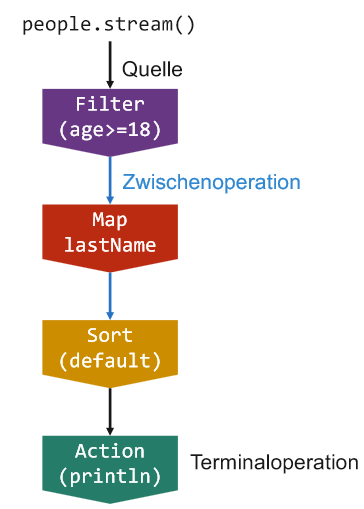
\includegraphics[width=\columnwidth,keepaspectratio=true]{Images/stream}
	\end{minipage}%%% to prevent a space
	\begin{minipage}{0.3\textwidth}
		\begin{lstlisting}
poeple.stream()
	.filter(p -> p.getAge() >= 18)
	.map(p -> p.getLastName())
	.sorted()
	.forEach(System.out::println);
		\end{lstlisting}
	\end{minipage}
\end{center}

\noindent\textbf{Wichtig:} Keine Interfernz, Collection darf \underline{nicht} verändert werden (1) oder Abhängikeiten zu äusseren, änderbaren Variablen haben (2) .
\begin{lstlisting}
// (1)
filter(p -> people.add(p))	
			
// (2)			
map(p -> {globalCounter++; return p;})	
\end{lstlisting}

\subsection{Operationen}
\begin{tabular}{p{4cm}p{5cm}}
	filter(Predicate) & Filtern mit Predicate-Funktionsobjekt/Lamda \\ \midrule
	map(Function) & Proijziert auf Rückgabewert von Funktionsobjekt/Lambda \\ \midrule
	mapToInt/Long/Double & Proijziert auf int,long,double \\ \midrule
	sorted() & Sortiert mit/Ohne Comperator \\ \midrule
	distinct() & Duplikate entfernen (equals()) \\ \midrule
	limit(long n) & Bis Element n liefern \\ \midrule
	skip(long n) & AB Element n liefern 
\end{tabular}